\chapter{Experimental Evaluations}

The main objective of the study was to compare how close the values from the low cost sensor network is to that of the reference system which is placed at the Plaza 400 building, downtown Prince George. The sensor system was deployed for six days from 30 May,2019 to 4 June, 2019 and was later compared to the values from reference system. In this chapter we will be discussing on the nature of the values and how close are these values to that of the reference system.

\section{Deployment}

In order to understand the accuracy and precison of our system, we deployed the air pollution monitoring system for eight days in University Heights, Prince George in which the first two days the system was put out for calibration and the rest six days for measurement. The figure \ref{deployed} shows the experimental set up of the sensor system deployed at the location. The system was directly connected to a power code and was made to hung over a platform. The collected values were transferred to the ThingSpeak database through the WiFi module (Wemos) in an hourly averaged form and hence 24 data set points were collected for each day.

\begin{figure}[h]
    \begin{center}
    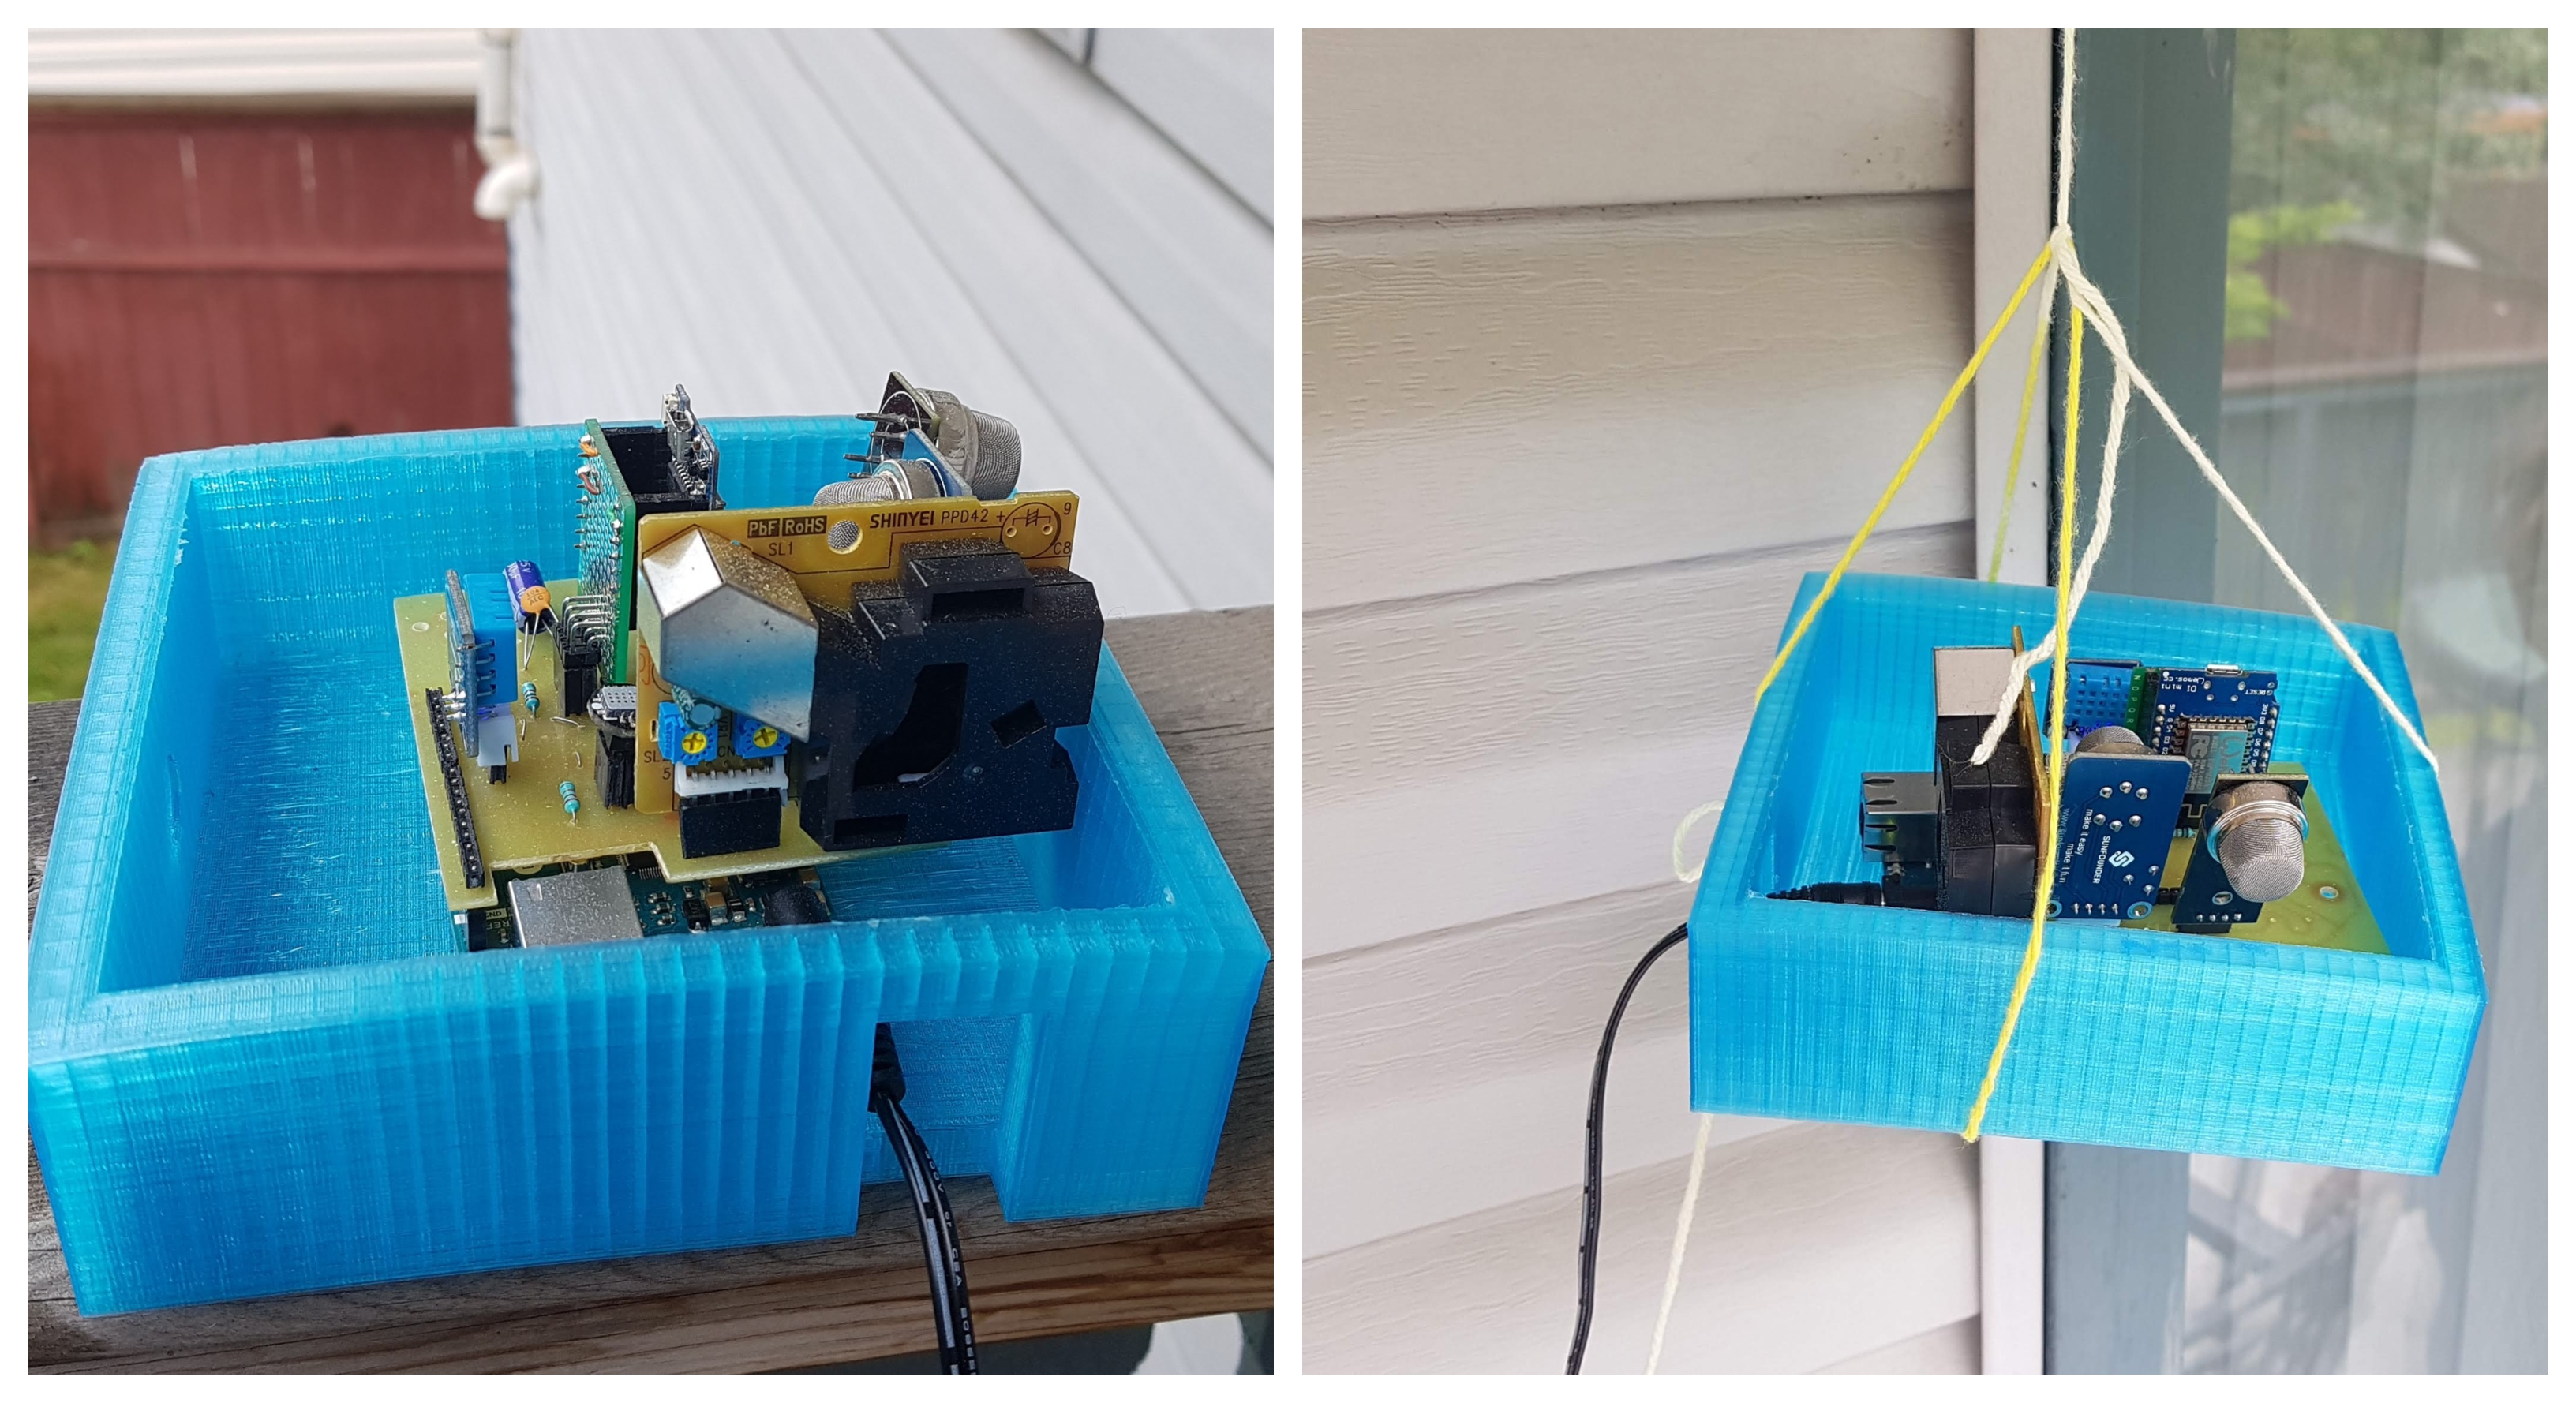
\includegraphics[scale=0.5]{images/figure20.jpg}
    \end{center}
    \caption{Deployed System at University Heights, Prince George}
    \label{deployed}

  \end{figure} 


  The main reason to conduct our deployment in this location was to have an easy access and to check on the system regularly in case of any sensor faults or signal distortions. The collected values in ThingSpeak database were compared to the reference values located in downtown Plaza 400 building except of carbon monoxide. The reference values for carbon monoxide were not found and hence were not analyzed. We have tried to analyze the daily variation of  Ozone, Particulate matter (both $PM_{2.5}$ and $PM_{10}$), Nitrogendioxide, temperature and humidity to their reference value.
\section{Calibration}

The sensors that we are using to measure the pollutants are low cost sensors and hence the sensitivity of these sensors are less compared to the monitoring station operated by local or state agencies. Inorder to boost the sensitivity of the low cost system and make it equivalent to the values from the monitoring stations we have tried to apply the calibration technique which is linear regression. By applying calibration technique the end result is a calibration curve which is obtained by fitting the most appropriate equation to the set of data \cite{Stone2001}. This calibration curve will be as close as to the true value or reference value in our case. We have attempted to calibrate our system by collecting the values for two days and then applying that calibration equation to the system. For each case we have shown the calibration curve as well as the regression fitting curve.

In figure \ref{calozone} shows the graph in which we have plotted three line graphs which includes the reference value from the monitoring station, our sensor value and also the calibration curve. The calibration curve was obtained by applying linear regression and extracting the regression fitting curve. From the line graph it can be clearly seen that the values from our sensor system has low sensitivity and after applying the calibration equation the graph is alligned to that of the reference system.


\begin{figure}[h]
  \begin{center}
  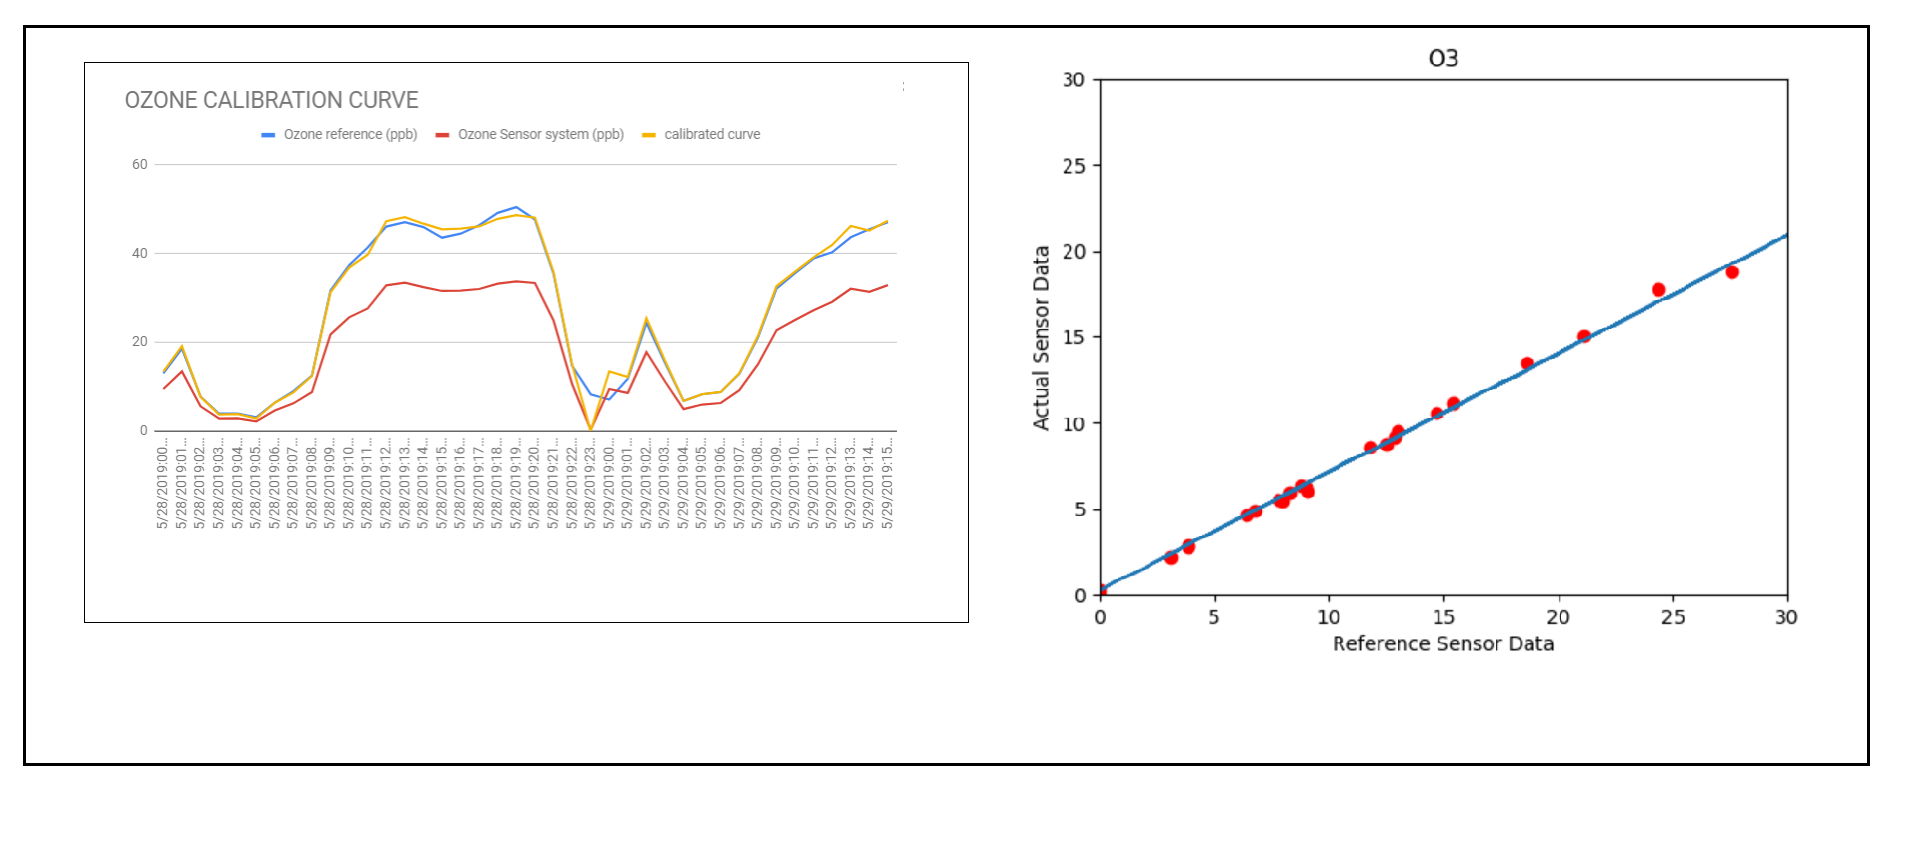
\includegraphics[scale=0.50]{images/figure36.png}
  \end{center}
  \caption{Calibration curve and the Regression fitting curve of Ozone}
  \label{calozone}
\end{figure}

The obtained calibration equation will be in the form of $ y = mx + c $ which shows a linear relationship equation. For each of the sensor a calibration equation waws obtained and is shown in the table \ref{tableequation}.
\begingroup
\setlength{\tabcolsep}{10pt} % Default value: 6pt
\renewcommand{\arraystretch}{1.5} % Default value: 1
\begin{table}[h]
  
  
  \begin{tabularx}{\columnwidth}{X|X}
      \hline
      Pollutant          & Regression equation    \\
      \hline
  
   
    
    




    
    $O_{3}$   & $y = 1.45162 * x + (-0.358)$ \\ 
    $NO_{2}$   & $y = 1.61757 * x + 0.03583$\\ 
    $PM_{2.5}$   & $y = 1.32472 * x + 0.13856$ \\ 
    $PM_{10}$   & $y = 1.62092 * x + (-0.39259)$\\ \hline
  
   
      
    
\end{tabularx}
 
  \caption{Regression equation for each sensor}
  \label{tableequation}
\end{table}
\endgroup
  \section{Data Analysis}
  In this section we will be comparing the collected data for each sensors and will be looking at the accuracy of these values. We will be using multiple line graph plots to observe the data and will be investigating if there is any variations to these data.
  
  \subsection{Ozone}

  The ground level ozone which is three atoms of oxygen ($O_3$) is not emmitted directly from any sources and is termed as a secondary pollutant. Our system measures this with the help of a semiconductor sensor MQ 131 which changes its conductivity with ozone \cite{technicalsheetozone}.The reference system in downtown uses an API model 400 ozone monitor for the city measurement\cite{Environment2010}.The figure \ref{Ozonesensor} shows the picture of the Ozone sensor used for measurement at the reference station as well as in our low cost sensor system.
  \begin{figure}[h]
    \begin{center}
    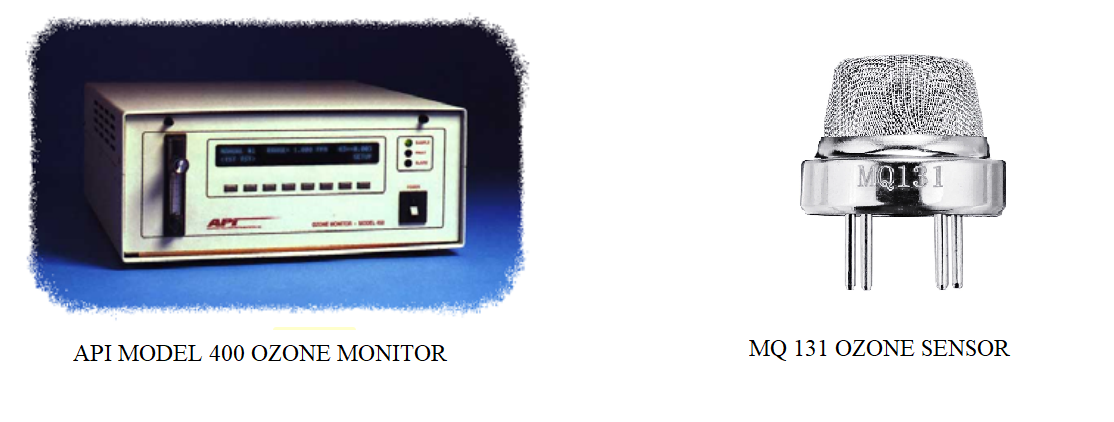
\includegraphics[scale=0.70]{images/figure30.png}
    \end{center}
    \caption{Ozone sensor used for measurement}
    \label{Ozonesensor}
  \end{figure}
  \bigskip

  
  From the collected data it can be identified that the content of Ozone gas during the day time is generally high due to the presence of other pollutant and is low during night. It can be seen from the graphs \ref{Ozone} and \ref{Ozone1} that our sensor was able to follow the trend similar to that of the reference system. During the first day of our measurement it can be noted that the value of Ozone from our system ranges for the day one ranges from 13.2 ppb in the early morning at 12:00 am and then the value decreases to  6.32 ppb at 5:00 am. After this the value keeps on increasing to 18.54 ppb at 8:00 am and later reaches its maximum to 55.09 ppb in the noon. From noon till night the value keeps on decresing to 38.47 ppb in the evening to 11.98 during the night. A similar trend is followed for all the days of observation. The maximum value obtained during the six days of observation from our system was 55.09 ppb at 12:00 pm on the first day and the reference system was showing a value of 62.90 ppb which records the maximum .

    
  \begin{figure}[h]
    \begin{center}
    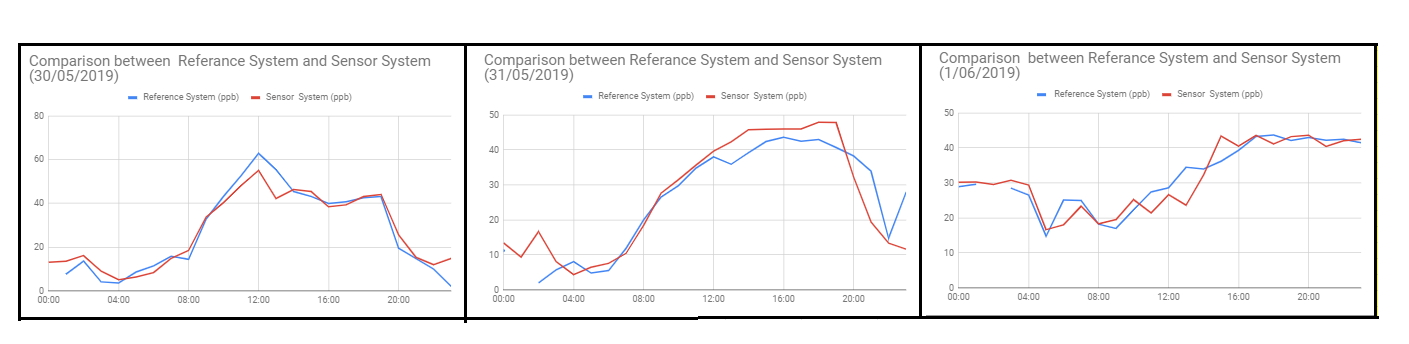
\includegraphics[scale=0.70]{images/figure21.png}
    \end{center}
    \caption{Comparison between Ozone values from sensor system and reference system from 30/05/2019 to 01/06/2019}
    \label{Ozone}
    \bigskip



  \end{figure}
  \bigskip
  \begin{figure}[h]
    \begin{center}
    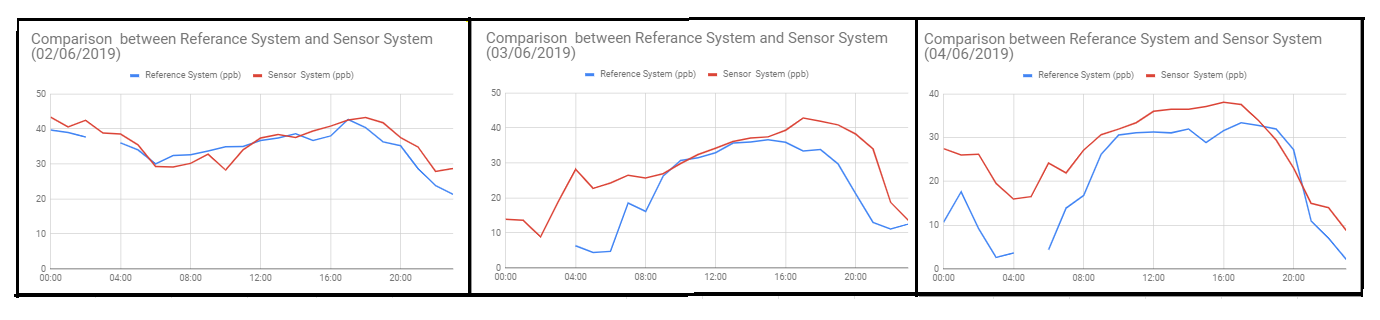
\includegraphics[scale=0.70]{images/figure22.png}
    \end{center}
    \caption{Comparison between Ozone values from sensor system and reference system from 02/06/2019 to 04/06/2019}
    \label{Ozone1}

  \end{figure}
  
The Graph \ref{Ozone} shows the line graphs of the first three days of the experiment and it can be seen that the values are very close to the refernce system. In the next figure \ref{Ozone1} shows the graphs for the next three days and it can be clearly seen that on the last two days the values from the sensor shows a slight variation when compared to the first three days. This can be interpreted in two ways, either it could be because the system needs to be recalibrated. The system might need to be updated with new regression equation so as to provide the graphs similar to the reference system. Secondly, we can also interpret this as a location specific effect. As the reference system is in downtown and there is a possibility of some activity which can cause a change in values or vice versa. Considering the fact that we are using a low cost sensor to measure the values from the sorrounding and hence the need for calibration should be considered as a priority. 







   \subsection{Nitrogen Dioxide}

 Nitrogen dioxide is found in urban areas which penetrates deep into lungs and causes pulmonary diseases.This gas is generated from liberation of Nitrogen present in the fuels and is considered as a serious pollutant in the environment \cite{Salonen2019} \cite{govcanada}. We have attempted to measure this pollutant with the help of low cost sensor. 
 
 $NO_{2}$ was measured with the help of a popular silicon gas sensor called as MICS-2714 by calculating the sensing resistance. The reference system located in Prince George plaza 400 is API $NO_{x}$ monitor \cite{Environment2010} which uses chemiluminesence principle to measure the pollutant . The figure \ref{Nitrogensensor} shows the image of both the sensors for detecting the pollutant.
   
   
   \begin{figure}[h]
    \begin{center}
    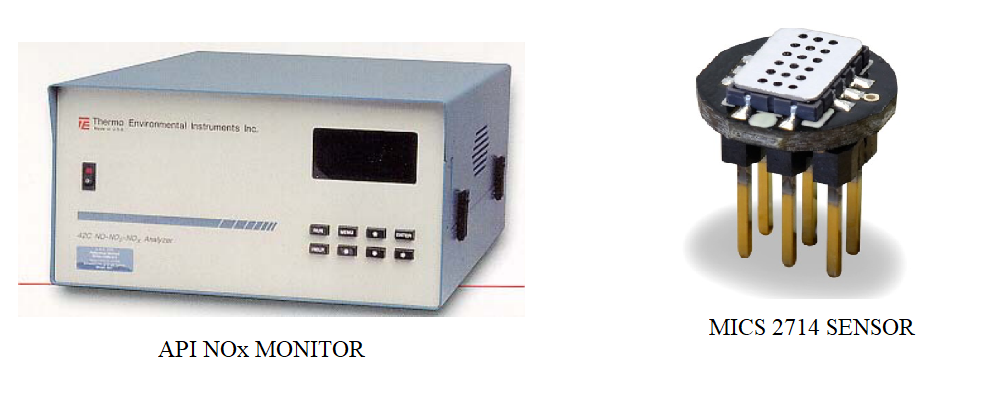
\includegraphics[scale=0.70]{images/figure31.png}
    \end{center}
    \caption{Nitrogen Sensor used for measurement}
  \label{Nitrogensensor}
\end{figure}
   
   
   
Using our sensor we have collected values and whave compared it to the values from the reference system. The graphical measurement values of the sensor in comparison with the reference system is shown in  the figure \ref{Nitrogen} and \ref{Nitrogen1}. 


   \begin{figure}[h]
      \begin{center}
      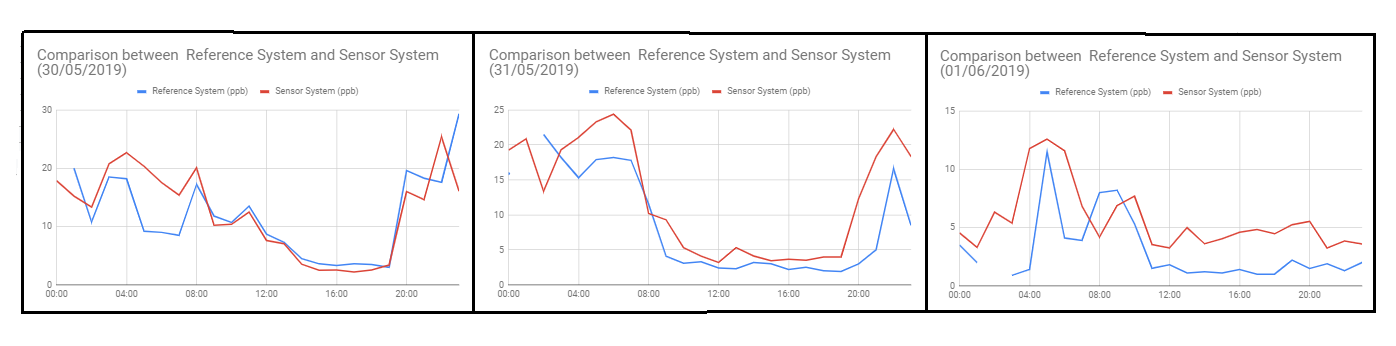
\includegraphics[scale=0.70]{images/figure23.png}
      \end{center}
      \caption{Comparison between Nitrogen Dioxide values from sensor system and reference system from 30/05/2019 to 01/06/2019}
    \label{Nitrogen}
  \end{figure}


  \bigskip

The maximum value measured from our sensor system was 25.39 ppb on the first day. The values measured from last two days comes under 12 ppb. The values are seen to be fluctualting through out the graphs. It can be interpreted from the graph that even though the values of the pollutant at each point of time is different from the reference system but for the first three days the trend is followed. At the same time it can also be seen in the figure \ref{Nitrogen1} that the values from both the system have less similarity.

    \begin{figure}[h]
      \begin{center}
      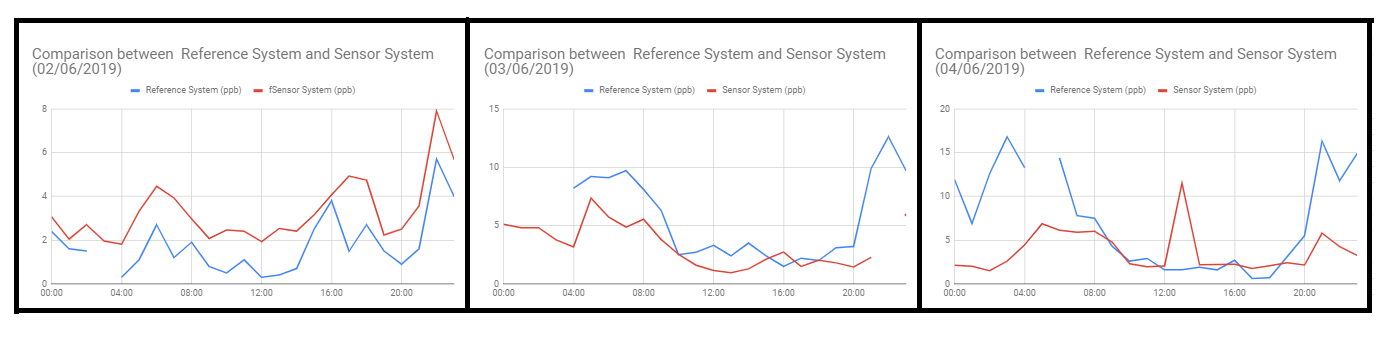
\includegraphics[scale=0.70]{images/figure24.png}
      \end{center}
      \caption{Comparison between Nitrogen Dioxide values from sensor system and reference system from 02/06/2019 to 04/06/2019}
      \label{Nitrogen1}
    \end{figure}

    On the first day our system measures a value of 22.67 ppb at 4:00 am and then the value decreases to around 10.23 ppb by 9:00 am and further decreases to 3.55 ppb at 2:00 pm. The measured value rises to around 16 ppb by 8:00 pm and by 11:00 pm the value is 25.39 ppb. It can be clearly seen from the graphs that the concentration of the Nitrogen oxide are high in the morning and then the slope comes down and again rises in the night. This variation of Nitrogen dioxide can be because of less or no  solar radiation in the early morning and late night \cite{Environment2010} \cite{George2005}. The less amount of energy from sun slows down the breakdown of Nitrogen Oxide to Nitric oxide which inturn increses the amount of Nitrogen oxides in the stratosphere \cite{EnvironmentalQualitySectionMoE2012} \cite{Environment2010}. This can be clearly seen in the graphs in both reference value as well as in our sensor value. Another reason for high values can also be related to heavy traffic as in the graph it clearly shows the concentration hits its peak around 8.00 am which is considered as an office time for most people in the city. The results from our observation shows that our sensor only shows the best measurement for the first two days and later the fluctuation in the concentration is high. This can be due to less sensitivity of the sensor used for measurement or might need better calibration method for the system.



\subsection{Particulate Matter}

The Particulate matters are those particles whose size ranges from 0.001$um$ till 100 $um$. The sources for the generation of this pollutant varies from town to town. In Prince George, pulp mills and saw mills are the primary source for their emission and during winter road dust also adds to the primary pollutant category as winter street sanding is done around that time \cite{Champagne1996}. The activities like street sweeping makes the particulate matter pollution even higher. The studies shows that the PM level are usually low during winter season and are higher during late winter and summer season \cite{EnvironmentalQualitySectionMoE2012}. In prince george particulate matter pollution is a serious concern and variety of studies are going under this category.

\begin{figure}[h]
  \begin{center}
  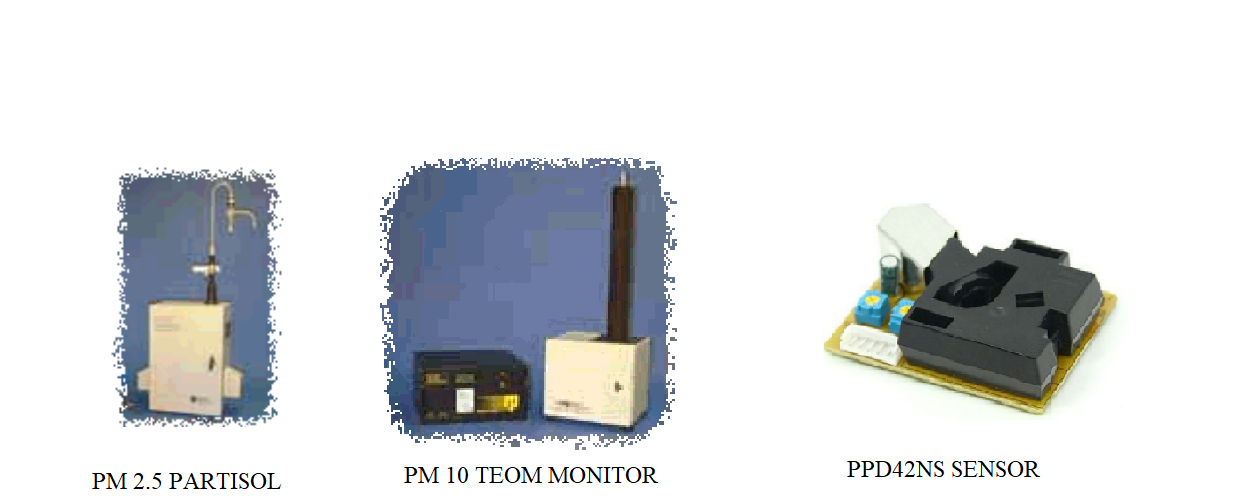
\includegraphics[scale=0.70]{images/figure29.png}
  \end{center}
  \caption{Particulate matter sensor}
\label{PM}
\end{figure}
\bigskip

 Measurement of Particulate matter was very tricky as there were a lot of options available in market and here we have used an optical sensor named PPD42NS which is a very low cost sensor that calculates the particle size using the principle of infrared. This sensor measures both $PM_{2.5}$ and $PM_{10}$ in an alternative manner. The reference system situated in downtown uses two different method for measurement, continuous and non-continuous \cite{EnvironmentalQualitySectionMoE2012}. Both the measurement method calculates the pollutant by drawing air from the atmosphere through an inlet and is placed on a teflon coated glass fibre filter  \cite{Environment2010}. The figure \ref{PM} shows the pictures of the sensors placed at downtown as well as sensor used for our system is shown.The comparison of both the measurement is done in the following section.

 \subsubsection{$PM_{10}$ and $PM_{2.5}$}
We have plotted the reference data from downtown to the collected data from the system. From the graph shown in the figure \ref{PM10} it can be seen that the values in the morning time especially from 6:00 am to 10:00 am is the highest for every day. On all the observed days the value of measurement did not exceed more than 100 $ug/m^3$. For the measured value from our system it can be seen that it shows a higher value than the Plaza 400 value. %The values from the reference system and our sensor system does not have many similarity this may be due to the location where the reference system is placed. 
This may be because the building which has the reference system is elevated above the ground and our sensor system are in ground level. This could be the reason why our system shows higher value than the reference system.
 During the year 1996 a short term experiment was conducted to understand if there is any difference in the street level pollution and was compared to the Plaza site (elevated building). The values collected from street levels shows that the particulate matter values were 30$\%$ higher than the Plaza value \cite{Environment2010}. 

 
 \begin{figure}[h]
  \begin{center}
  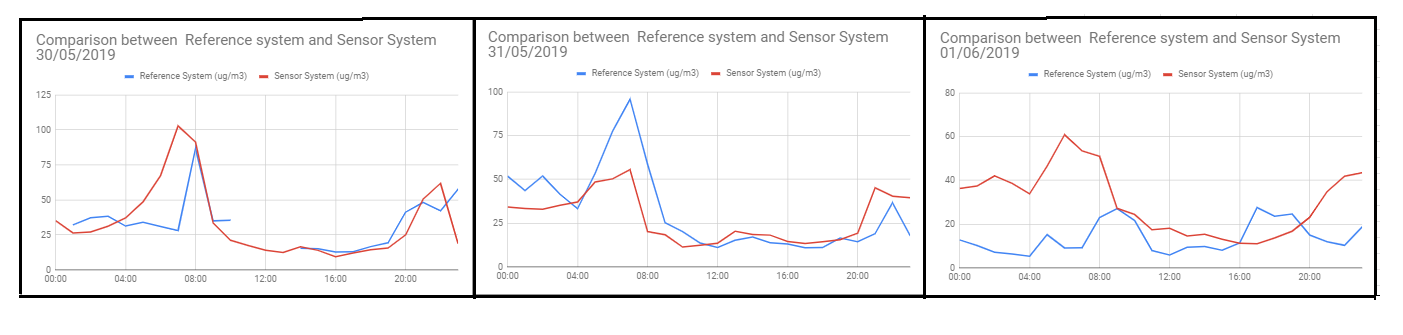
\includegraphics[scale=0.70]{images/figure25.png}
  \end{center}
  \caption{Comparison between $PM_{10}$ values from sensor system and reference system from 30/05/2019 to 04/06/2019}
\label{PM10}
\end{figure}
\bigskip


  Another factor to be taken into account is  the location where our sensor is placed and the wind direction. These factors causes variation to the values which makes the graph looks different. Also as the sensor was placed outside a house in uptown there could be activities which happened inside the house such as cooking, vaccuming, smoking etc might have caused these variations. %From the graph it can be clearly seen that during the day time the values of $PM_{10}$ is generally low for all the six days.
 The graph for $PM_{10}$ shows that the during the day time especially from 8:00 am to 4:00 pm on every day the pollutant level is low on the measured day. This is true in the case of the reference value as well.

The factors which contributed to $PM_{10}$ are similar to that for $PM_{2.5}$ like combustion, road dust, industries etc. The particle size of $PM_{2.5}$ are more finer than $PM_{10}$ and has more health effects. On inhaling these particles can causes cardivascular diseases and other breathing problem. From the graph shown in figure \ref{PM2.5} it can be seen very clearly that on all the measured day the values are low and have not exceeded 40 $ug/m^3$. The reason for such low values can be also related to meterological factor, wind direction or the location where it is measured. The graphs for $PM_{2.5}$ shows a good similarity to the reference system values.

%Both $PM_{2.5}$ and $PM_{10}$ are location dependent sensor which means the value of the pollutant very much changes with the activity that is occuring near the sensor.


\begin{figure}[h]
  \begin{center}
  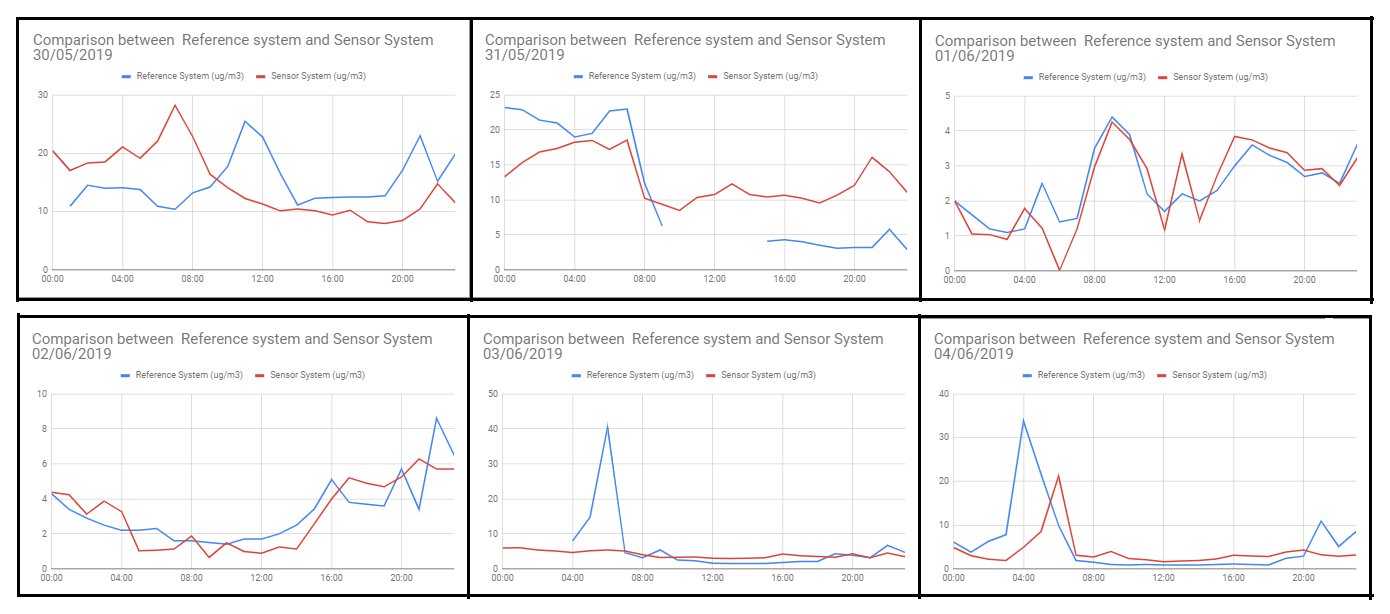
\includegraphics[scale=0.70]{images/figure27.png}
  \end{center}
  \caption{Comparison between $PM_{2.5}$ values from sensor system and reference system from 30/05/2019 to 01/06/2019}
\label{PM2.5}
\end{figure}

Unlike $PM_{10}$  the values for $PM_{2.5}$ does not have a regular pattern in the graph. On the first two days the values from the graph showed a higher value in the morning and relatively lower values during the evening and night. On the third day the graph shows some hikes in the value during noon and the evening time. This could be related to some activities that might have occured in the location of the sensor system. On the last three days the pollutant level could be seen as low for the entire day. This is very tricky to identify, unlike other pollutants present in the atmosphere both $PM_{10}$  and $PM_{2.5}$ pollutant level are very dependent on location and any small activities could make the values go high or low.


\subsection{Indexes}

The indexes are the numbers which makes the general public understand more about the air quality in the area they live in. In our analysis we have attempted to compare the AQI (Air Quality Index) and AQHI (Air Quality Health Index) indexes from the collected values of both the system.

In Canada the most popular index for the public is AQHI is a number scale which defines how the air quality affects the human health \cite{AQHICAN}. The pollutants which are included for the calculation of the health index are $NO_{2}$, $PM_{2.5}$ and $O_{3}$. In our graph we have calculated the health index for each hour and then we took the average for the day and have compared it with the averaged health index data provided by the government. The value of AQHI ranges from 1 to 10+ (highest). The figure \ref{AQHIAV} shows the bar graph which compares both the values. 
\begin{figure}[h]
  \begin{center}
  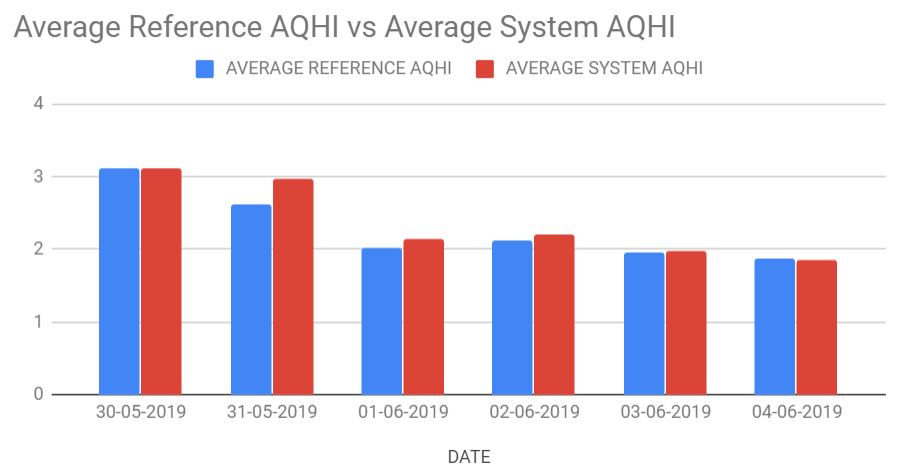
\includegraphics[scale=0.70]{images/figure34.png}
  \end{center}
  \caption{Comparison between average AQHI from both Reference and Sensor System}
  \label{AQHIAV}
\end{figure}

 The first day both the average AQHI from the reference system and the sensor system gives almost equal value which are 3.12 and 3.11 respectievely. On the next three days our system showed a higher AQHI value than the reference system and on the last two days the averaged AQHI value is same as that to the average reference system. This change in value is because of the variation in readings of the measured pollutant discussed above. On all the measured days the risk factor associated with health is low as per the index chart provided by the government \cite{AQHICAN}.

 The next index that we calculated is AQI in which we have used the same set of pollutant that we have used for the computations of AQHI. This index shows how polluted the vicinity is by giving the public a value between 0 to 400+ (highest). Here we have again used the average value for both the measuring system. The figure \ref{AQIAV} shows the graph of the averaged AQI values.

 \begin{figure}[h]
  \begin{center}
  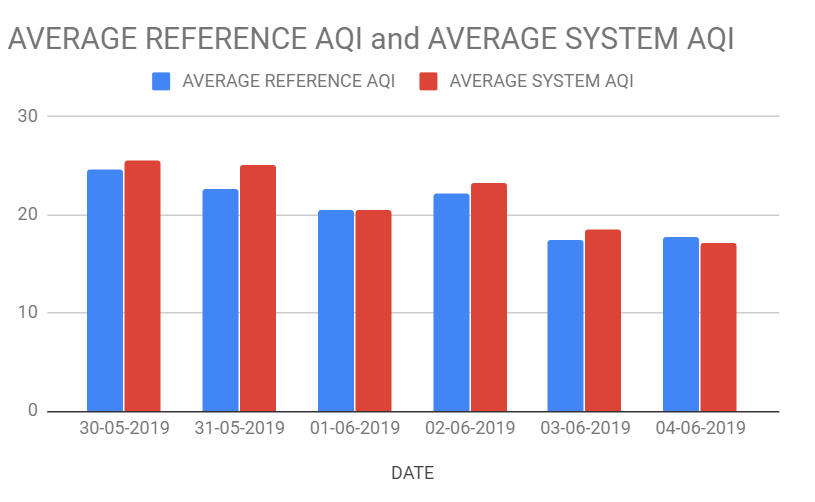
\includegraphics[scale=0.70]{images/figure35.png}
  \end{center}
  \caption{Comparison between average AQI from both Reference and Sensor System}
  \label{AQIAV}
\end{figure}

It can be seen that on majority of the days our sensor system shows a higher AQI value when compared to the reference system except on the last day. This can again be related to the alteration in the observed value from the reference. These averaged values falls into the first category of the scale provided by the government which means the air quality during the measured days was 'Good'. For the calculation of AQI we have not included Carbon monoxide and $PM_{10}$ as well. 
Having a look at both the graphs it shows how well the system could capture the values after calibration. 

These are the observation which we have obtained after we have put our system out for six days. The system worked very close to the reference system after the calibration except for Particulate matter. Further in the next chapter, I will be proposing on few suggestions which could be done to the system.